图~\ref{fig:cnn-transform-algorithms}把三类变换放在同一条输入、乘法和恢复路径上；它们的区别在于坐标的选择与要恢复的输出。

\begin{figure*}[tb]
  \centering
  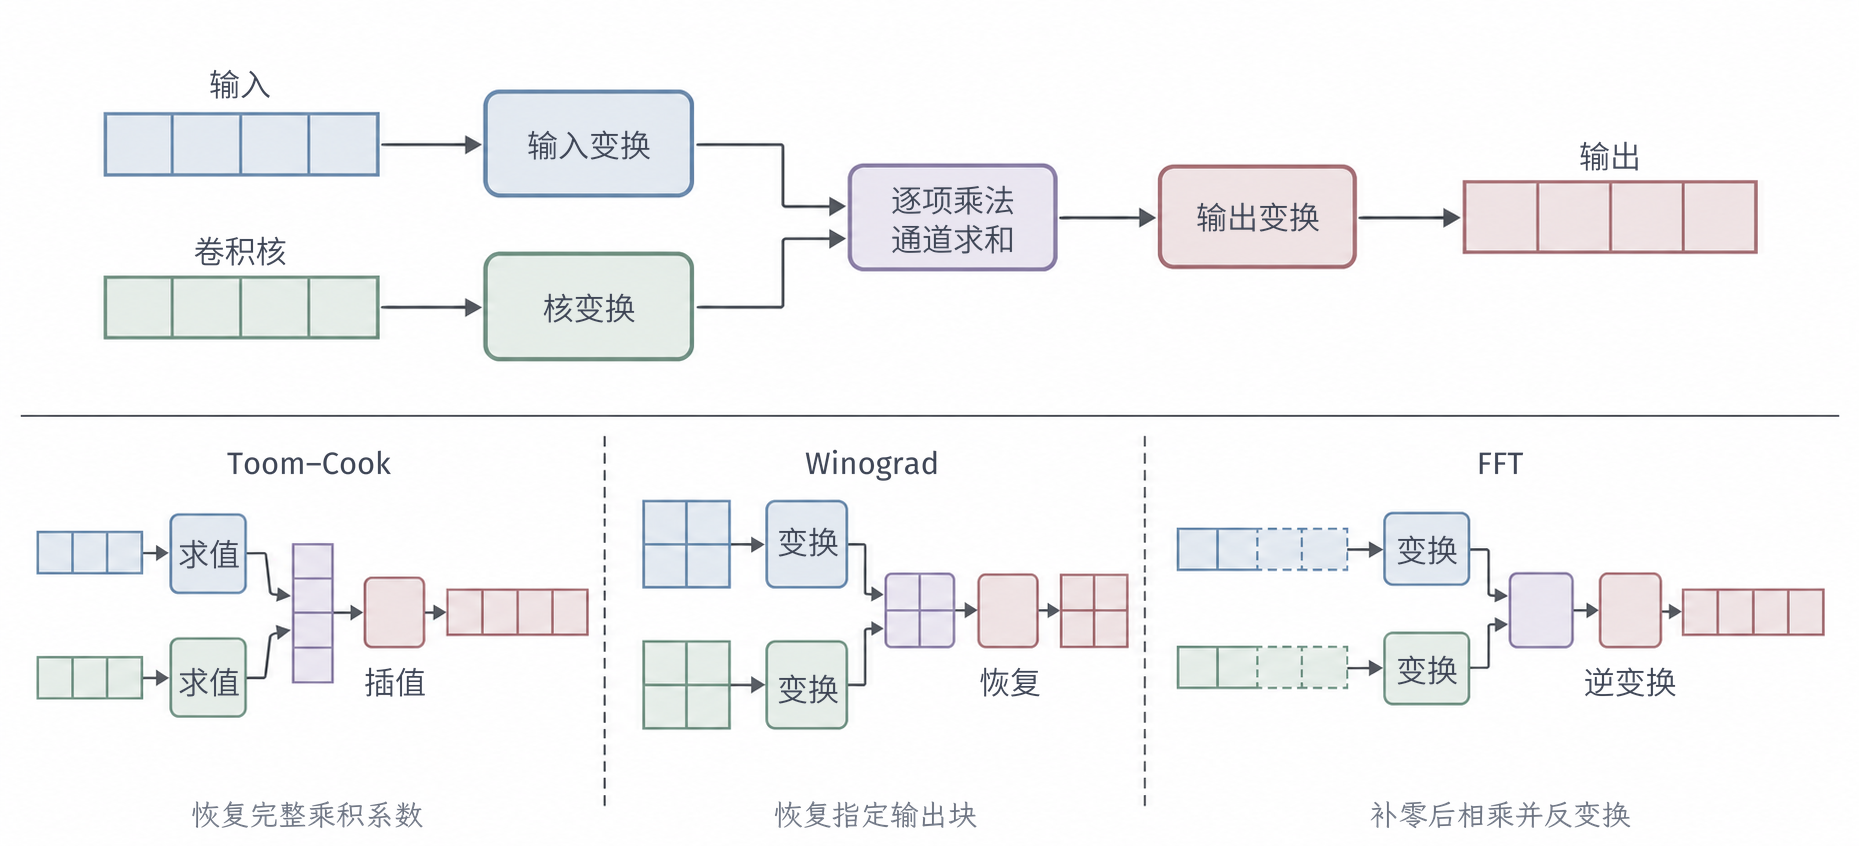
\includegraphics[width=169mm]{figures/01-mathematical-preliminaries/03-graphs-and-signals/generated/cnn-transform-algorithms/figure.png}
  \caption{变换类卷积的共同流程与不同目标。Toom--Cook通过多项式求值及插值恢复完整乘积系数；Winograd通过固定小矩阵恢复所需输出块；FFT在补零后的频域相乘并反变换。输入和核可以分别变换，变换结果按输入通道相乘并求和；能复用多少次，决定变换开销能否被摊薄。格子只示意数组，不表示具体尺寸或数值。}
  \label{fig:cnn-transform-algorithms}
\end{figure*}
